\documentclass[11pt]{article}
\usepackage{graphicx}    % needed for including graphics e.g. EPS, PS
\topmargin -1.5cm        % read Lamport p.163
\oddsidemargin -0.04cm   % read Lamport p.163
\evensidemargin -0.04cm  % same as oddsidemargin but for left-hand pages
\textwidth 16.59cm
\textheight 21.94cm 
%\pagestyle{empty}       % Uncomment if don't want page numbers
\parskip 7.2pt           % sets spacing between paragraphs
%\renewcommand{\baselinestretch}{1.5} % Uncomment for 1.5 spacing between lines
\usepackage{amsmath}
\usepackage{amsfonts}
\usepackage{verbatim}
\parindent 0pt		 % sets leading space for paragraphs
\author{Erik Waingarten \and Fermi Ma}
\title{Taking Dual}


\begin{document}         
\maketitle

Suppose we are given a set of $n$ points $a_i = (x_i, y_i)$ in the $xy$ plane. Then we can think of the grid in the plane formed by all horizontal and vertical lines going through the points $a_i$. Note that since there are at most $n$ different $x$ values and $n$ different $y$ values, there are $n^2$ intersection points to consider (it is not hard to see that we only need these intersection points). We construct indicator variables $b_{jk}$, where $b_{jk} = 1$ if the grid point in the $j$th row and $k$th column is present, and 0 otherwise. Thus, the problem can be restated as an integer linear program (ILP) where the objective is:

\[ \min \sum_{j,k} b_{jk} \]

subject to the following constraints:
\begin{align}
\sum_{\text{points on the edges of the rectangle }a_i, a_j} b_{kl} &\geq 1 \hspace{.3in} \forall \hspace{.1in} \text{valid rectangles} \hspace{.1in} a_i, a_j\\
b_{ij} + b_{kl} - \sum_{\text{points in edge of rectangle }b_{ij}, b_{kl}} &\leq 1 \hspace{.3in}  \forall \hspace{.1in} \text{valid rectangles} \hspace{.1in} b_{ij}, b_{kl}
\end{align}

We can write this more concisely as an LP as
\[ \min \sum b_{jk} \]
such that:
\begin{align}
 b_{x_iy_i} = 1 \hspace{.3in} \forall a_i = (x_i, y_i)
\end{align}

\begin{align}
b_{ij} + b_{nm} - \left(\sum_{l=i+1}^{n-1} (b_{lj}+b_{lm}) + \sum_{l=j+1}^{m-1} (b_{il} + b_{nl}) + b_{im} + b_{nj} \right) &\leq& 1 & \hspace{.3in} \forall i<n, j<m \\
b_{im} + b_{nj} - \left(\sum_{l=i+1}^{n-1} (b_{lj}+b_{lm}) + \sum_{l=j+1}^{m-1} (b_{il} + b_{nl}) + b_{ij} + b_{nm} \right) &\leq& 1 & \hspace{.3in} \forall i<n, j<m
\end{align}
Where constraint (3) makes sure that all the points are counted, constraint (4) makes sure that all ``positive rectangles are accounted", and (5) makes sure all ``negative" rectangles are accounted. 

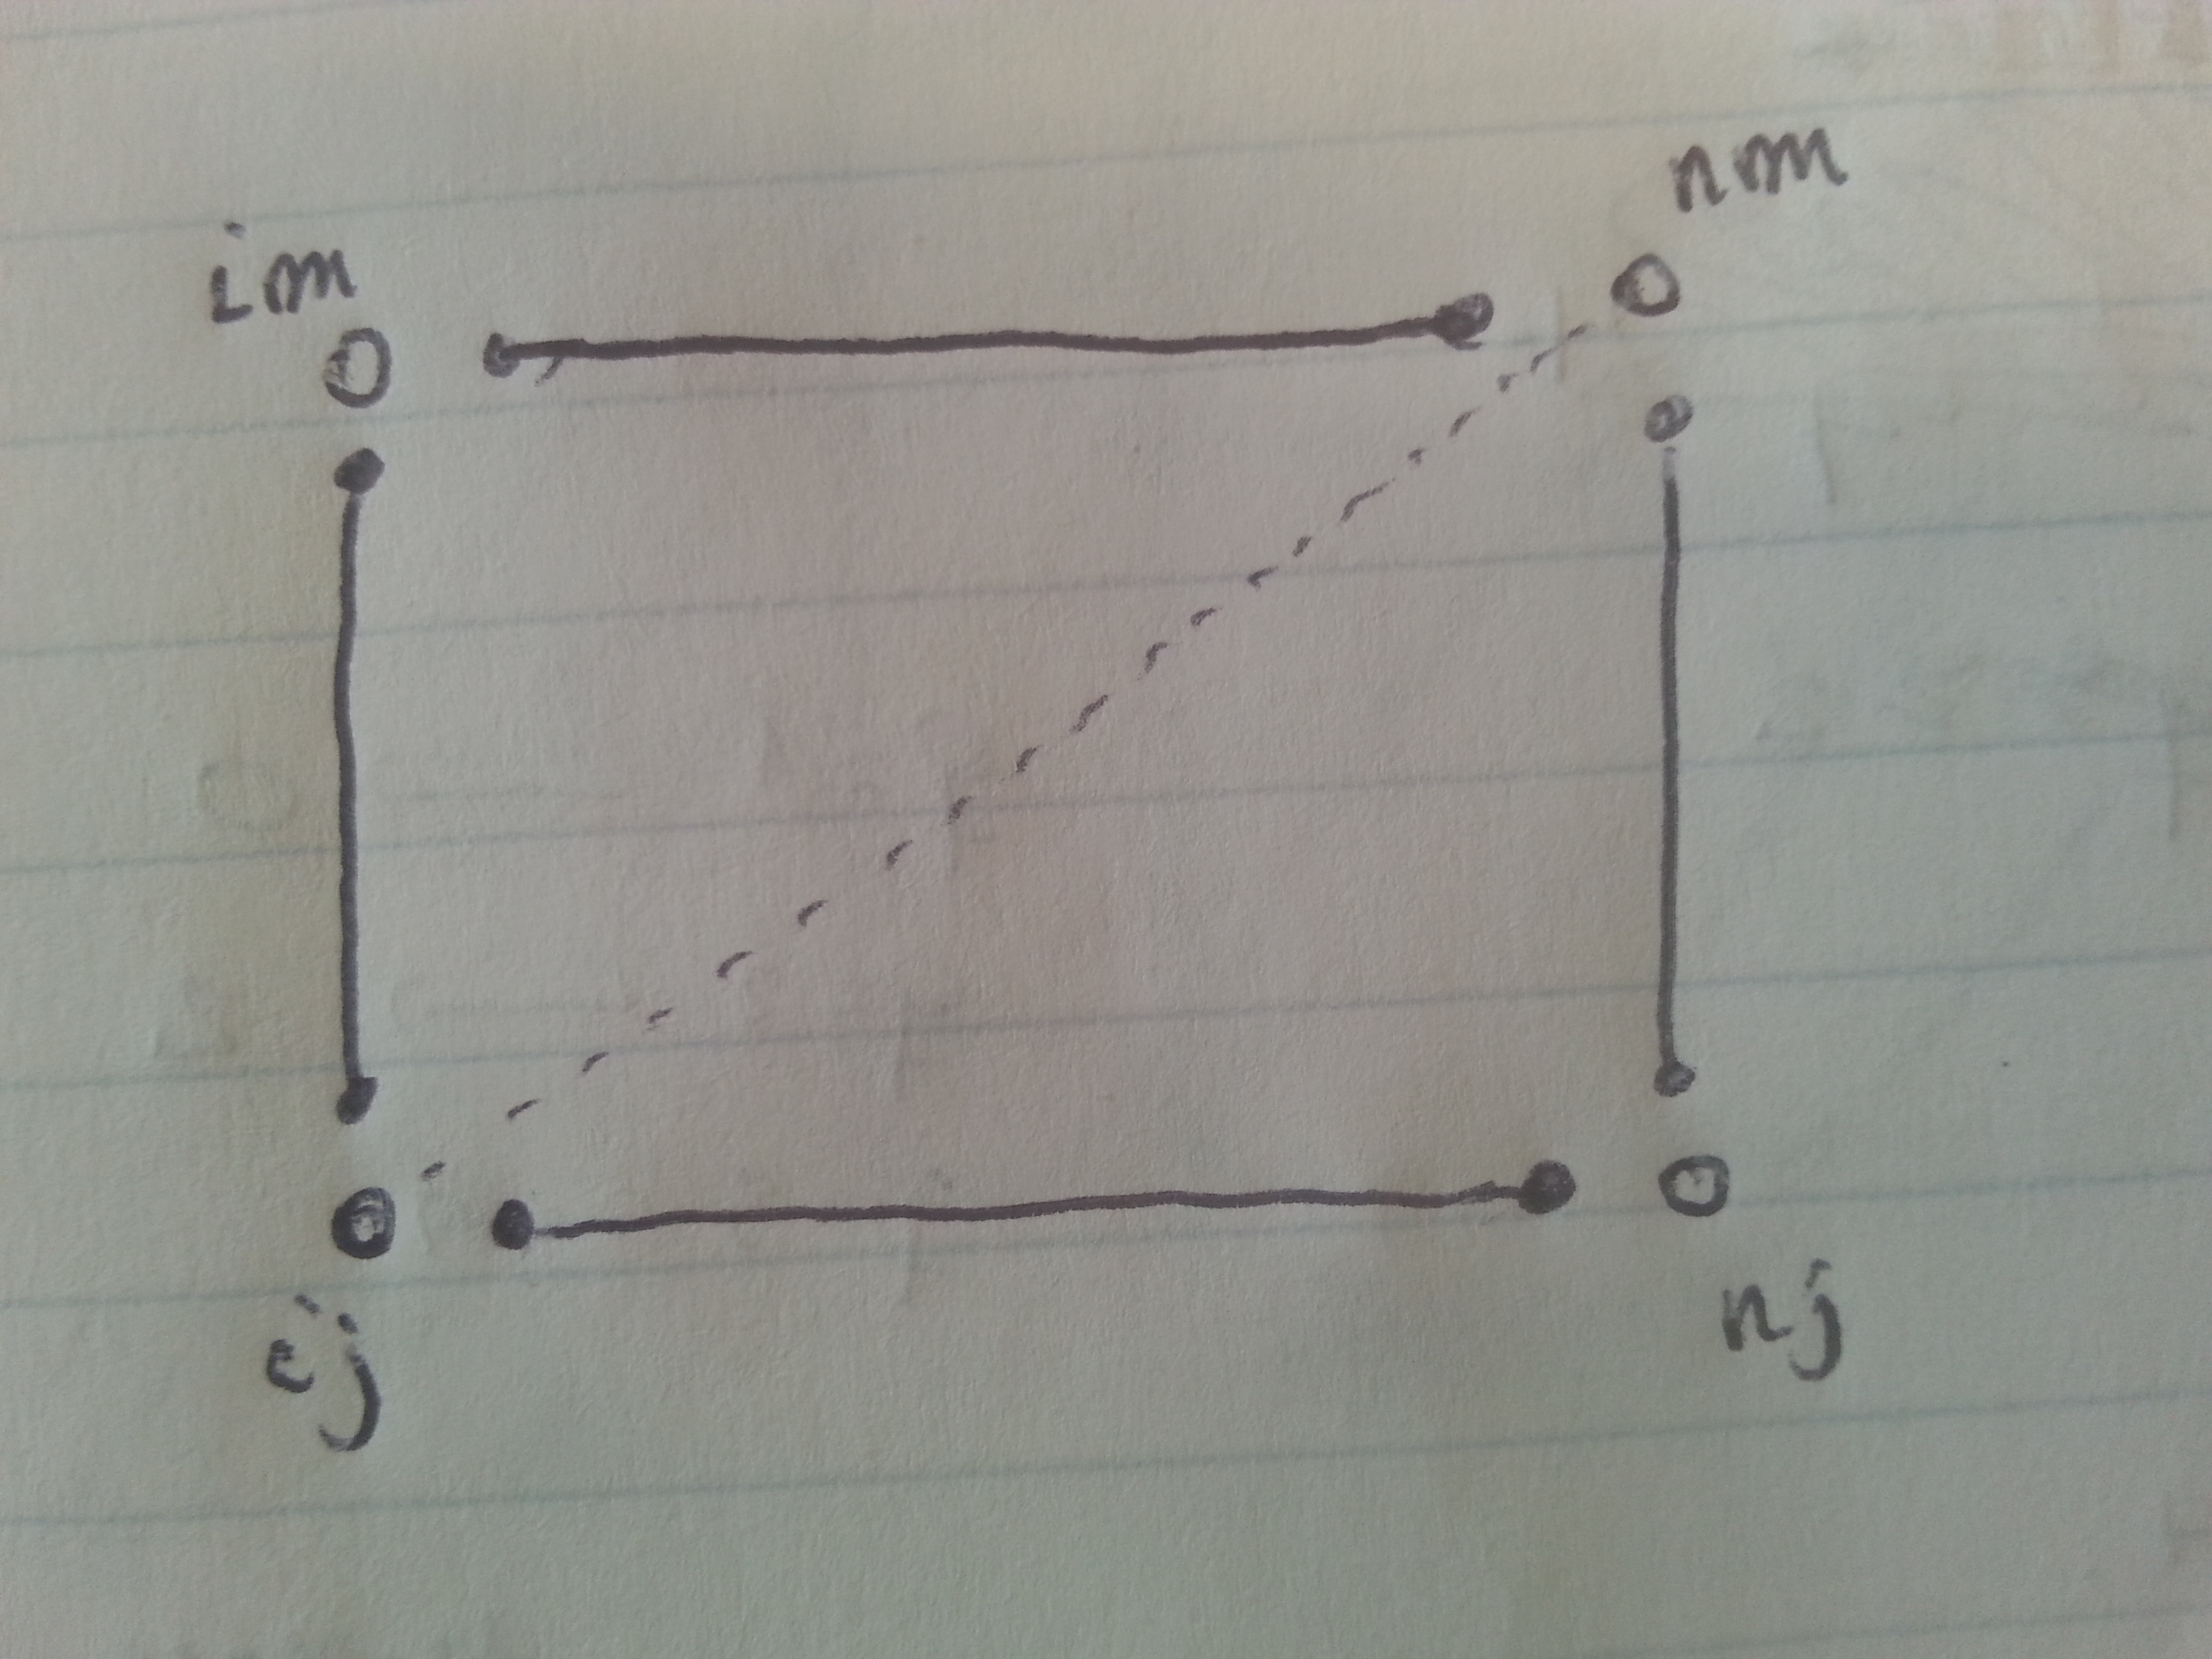
\includegraphics[height=200px, width=200px]{positiverectangle.jpg}

The above figure is an example of the rectangle covered by (4), where the lines represent those points covered by the sums. 

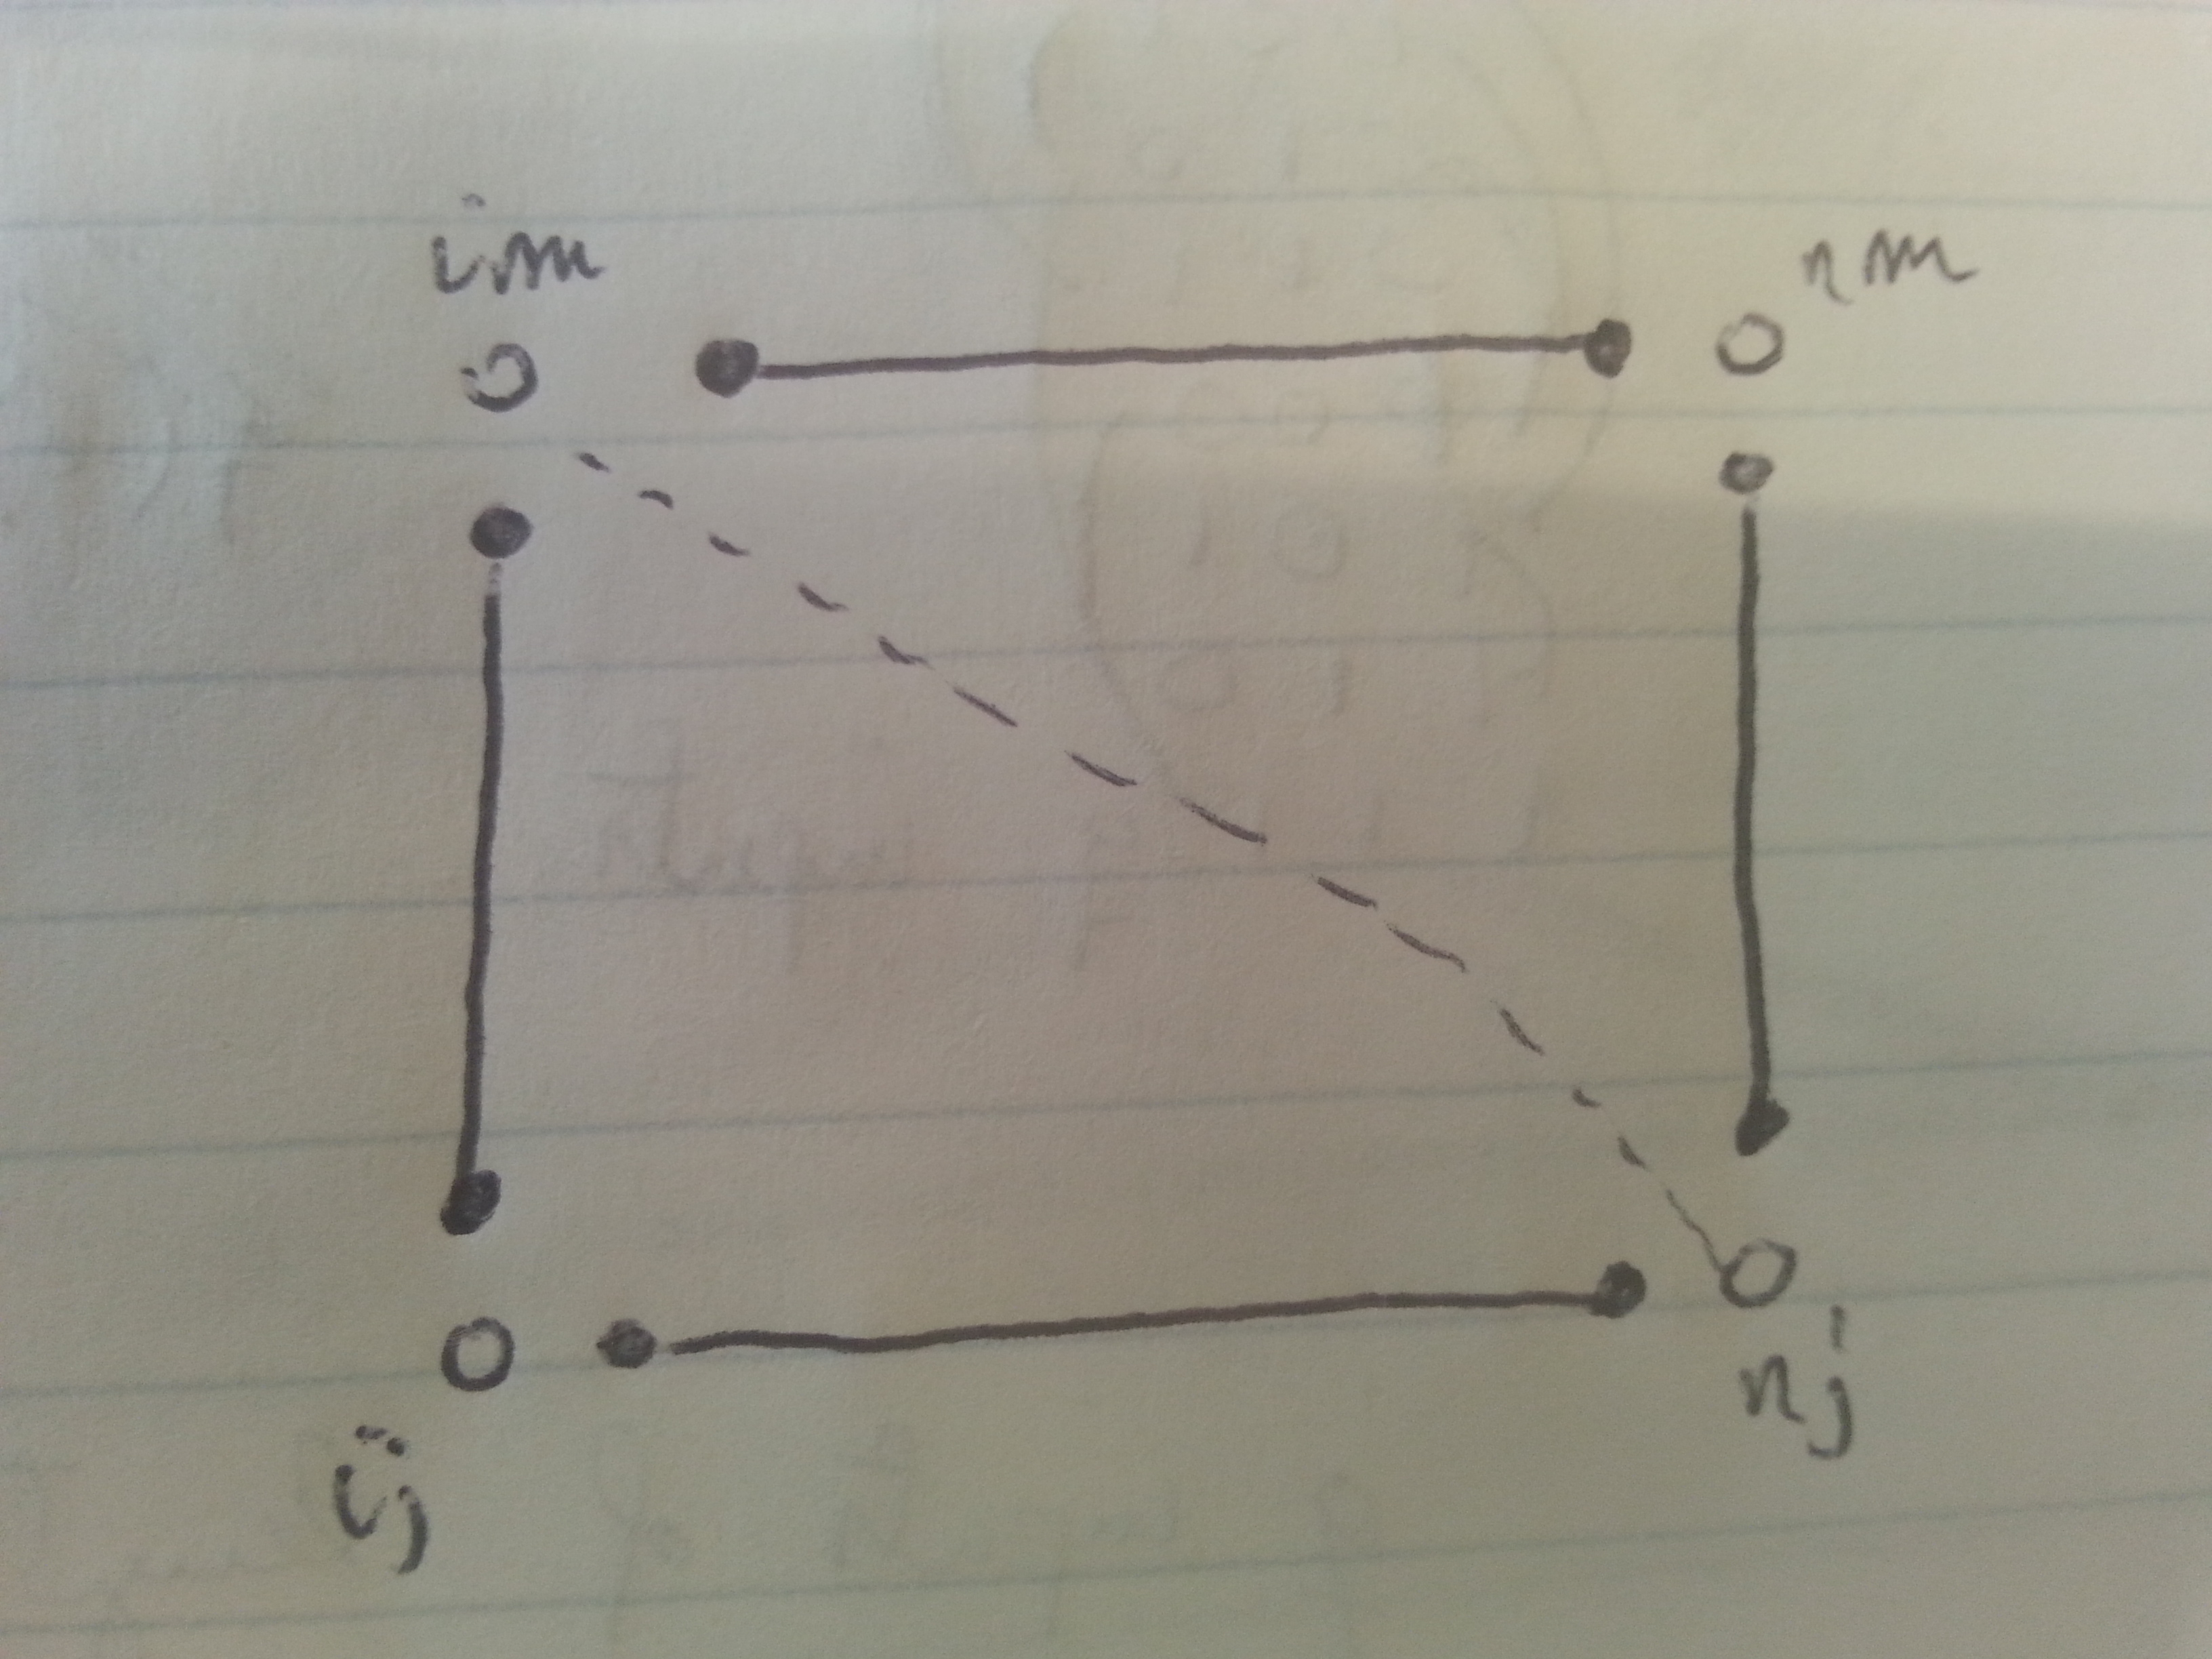
\includegraphics[height=200px, width=200px]{negativerectangle.jpg}

The above figure is similar to the previous one, except that this is the negative rectangle. 

We can represent the linear program as a matrix, which will make it easier to take its dual:
\[ \min \hspace{.1in} [ \begin{array}{cccc} 1 & 1 & \dots & 1 \end{array} ] \left[\begin{array}{c} b_{11} \\ b_{12} \\ \vdots \\ b_{nn} \end{array} \right]\]
such that
\[ \left[ \begin{array}{c} \vdots \\ \text{ $P$ = positive rectangles } \\ \vdots \\ \text{ $N$ = negative rectangles } \\ \vdots \\ \text{ $I_n$ = equality } \end{array} \right] 
\left[\begin{array}{c} b_{11} \\ b_{12} \\ \vdots \\ b_{nn} \end{array} \right] 
\begin{array}{c} \\ \leq \\ \\ \\ \leq \\ \\ \\ = \end{array} 
\left[\begin{array}{c} 1 \\\\ 1 \\\\ \vdots \\\\ 1 \end{array} \right] \]

Where $P$ and $N$ are $\dbinom{n}{2}^2 \times n^2$ matrices, since there are that many positive and negative rectangles. And $I_n$ is the identity matrix. Furthermore, we require that all variables are positive. 

So we can take the dual:
\[ \max y^T \left[ \begin{array}{c} 1 \\ 1 \\ \vdots \\ 1 \end{array} \right] \]
such that
\[ \left[ \begin{array}{ccc} \vdots & \vdots & \vdots \\
					  P^T & N^T & I_n \\
					\vdots & \vdots & \vdots \end{array} \right] y
\leq  \left[ \begin{array}{c} 1 \\ 1 \\ \vdots \\ 1 \end{array} \right] \]
Where the first $n$ variables in $y$ can take on any value, and the rest must all be negative. 

This will corresponds to the following:

We will have a variable for each positive rectangle and each negative rectangle, denoted $b_{ij, lk}$ and a variable for each point that was set $a_{xy}$. Then for each point $xy$, if $xy$ is set, then we have the following constraint:
\[ a_{xy} + \sum_{\text{ rectangles where $xy$ on corner }} b_{ij, lk} - \sum_{\text{ rectangles where $xy$ on side }} b_{ij,lk} \leq 1 \]
If $xy$ is not set, then the $a_{xy}$ term is not present. We want to maximize
\[ \sum a_{xy} + \sum b_{ij,lk} \]
where $b_{ij,lk} \leq 0$. And the $a$'s are unconstrained. In some sense, we would like to set the values of the rectangles that have points two points on their corners as negative, since then we could raise $a_{xy}$ by the same amount in both corners and thus increase the objective.
\end{document}
